%!TEX root = ..\Master.tex

\subsection{Support Vector Machines}
The support vector machine is a supervised learning algorithm.
Compared to neural network, it sometimes gives a cleaner and more powerful way of learning complex non-linear functions. (TODO: What does more powerful mean?)

\subsubsection{Linear}
When doing the linear classifier, SVM will try to find the line that seperates the data with the highest margin as seen on figure \ref{fig:svm-margin}.

\begin{figure}[H]
\centering
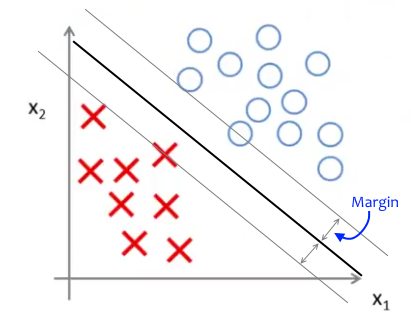
\includegraphics[scale=.75]{billeder/svm-margin}
\caption{Large margin classification.}
\label{fig:svm-margin}
\end{figure}

By solving the optimization problem defined as equation \ref{eq:svm-linear-optimization}, we find the parameters for the linear SVM classifier.
\begin{equation}
\min_{\theta}C \sum_{i=1}^{m}
\left[ y^{(i)}cost_1(\theta^Tx^{(i)})+(1-y^{(i)})cost_0(\theta^Tx^{(i)}) \right]
+ \frac{1}{2}\sum_{i=1}^{n}\theta^2_j
\label{eq:svm-linear-optimization}
\end{equation}
We must choose the value of the constant $C$. (TODO: what is its effect? Some regularization thing.)
Figure \ref{fig:svm-cost-function} shows the plot of $cost_0$ and $cost_1$.
\begin{figure}[H]
\centering
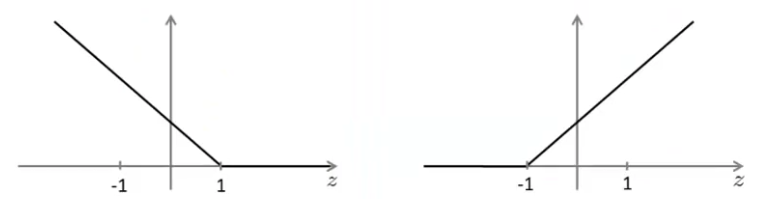
\includegraphics[scale=.75]{billeder/svm-cost-function}
\caption{Left: $cost_1(\theta^Tx^{(i)})$. Right: $cost_0(\theta^Tx^{(i)})$}
\label{fig:svm-cost-function}
\end{figure}

Hypothesis: (TODO: Is this correct? shouldn't it be 1 if $\theta^Tx \geq 1$ and 0 if $\theta^Tx \leq -1$)
\begin{equation}
h = 
\begin{cases}
1 & \text{if}\ \theta^Tx \geq 0 \\
0 & \text{otherwise}
\end{cases}
\end{equation}

\subsubsection{Non-linear}
Finds the kernels that seperates the data best.
gaussian kernels.

\begin{figure}[H]
\centering
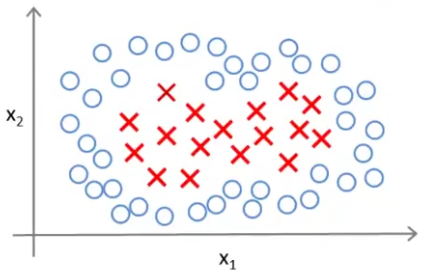
\includegraphics[scale=.75]{billeder/svm-non-linear}
\caption{Example of problem that requires non-linear classification.}
\label{fig:svm-non-linear}
\end{figure}

The gaussian kernel function:
\begin{equation}
f_i = similarity(x,l^{(i)}) =
exp\left(-\frac{||x-l^{(i)}||^2}{2\sigma^2}\right)
\end{equation}

At each training example we will put a landmark:
\begin{equation}
\begin{split}
\text{Given}\ (x^{(1)},y^{(1)}),(x^{(2)},y^{(2)}),\dots,(x^{(m)},y^{(m)}),\\
\text{choose}\ l^{(1)} = x^{(1)},l^{(2)} = x^{(2)},\dots,l^{(m)} = x^{(m)}
\end{split}
\end{equation}

We convert the training data into new feature vectors. For training example $(x^{(i)},y^{(i)})$:
\begin{equation}
f^{(i)}=
\begin{bmatrix}
f_0^{(i)} \\
f_1^{(i)} \\
\vdots \\
f_m^{(i)}
\end{bmatrix}
\end{equation}
 where $f_0^{(i)} = 1$.

The minimization problem now looks like:
\begin{equation}
\min_{\theta}C \sum_{i=1}^{m}
\left[ y^{(i)}cost_1(\theta^Tf^{(i)})+(1-y^{(i)})cost_0(\theta^Tf^{(i)}) \right]
+ \frac{1}{2}\sum_{i=1}^{m}\theta^2_j
\end{equation}

A large C gives lower bias and high variance, which means it uses a smaller amount of regularization and is more prone to overfitting. \\
A small C gives higher bias and low variance, which means it uses a higher amount of regularization and is more prone to underfitting. \\
A large $\sigma^2$ gives higher bias and lower variance, which means that features $f_i$ varies more smoothly. \\
A small $\sigma^2$ gives lower bias and higher variance, which means that features $f_i$ varies less smoothly.

(TODO: How do we use it?)

%------------------------------------------------